% begin module derivative-sine-graph
\begin{frame}
\frametitle{(3.4) Derivatives of Trigonometric Functions}
\ \only<handout:0| 1>{%
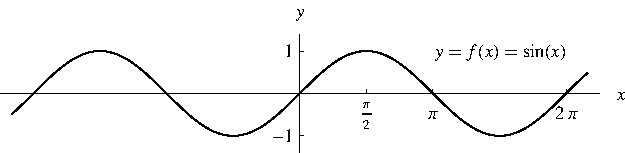
\includegraphics[width=12cm]{derivatives-trig/pictures/03-04-sina.pdf}%
}%
\only<handout:0| 2-3>{%
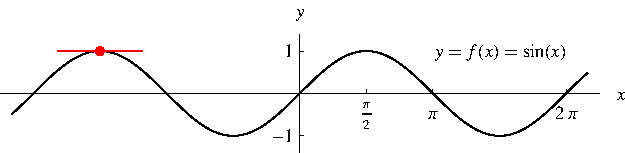
\includegraphics[width=12cm]{derivatives-trig/pictures/03-04-sinb.pdf}%
}%
\only<handout:0| 4-5>{%
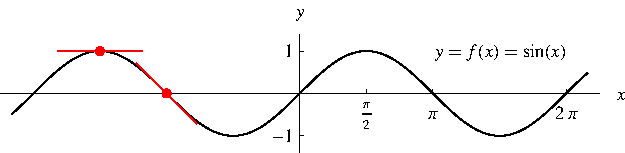
\includegraphics[width=12cm]{derivatives-trig/pictures/03-04-sinc.pdf}%
}%
\only<handout:0| 6-7>{%
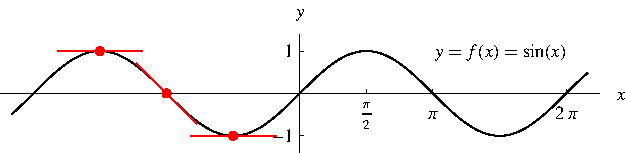
\includegraphics[width=12cm]{derivatives-trig/pictures/03-04-sind.pdf}%
}%
\only<handout:0| 8-9>{%
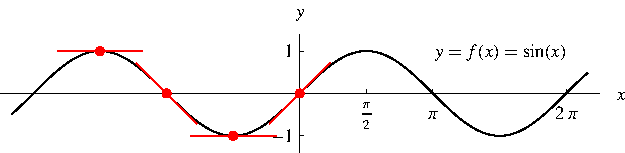
\includegraphics[width=12cm]{derivatives-trig/pictures/03-04-sine.pdf}%
}%
\only<handout:0| 10-11>{%
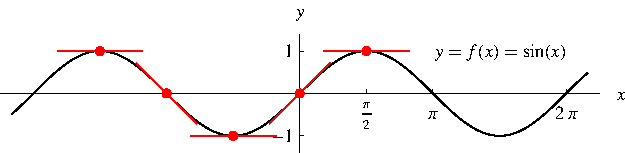
\includegraphics[width=12cm]{derivatives-trig/pictures/03-04-sinf.pdf}%
}%
\only<handout:0| 12-13>{%
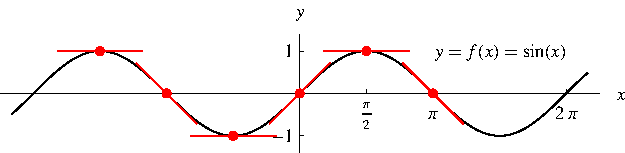
\includegraphics[width=12cm]{derivatives-trig/pictures/03-04-sing.pdf}%
}%
\only<14->{%
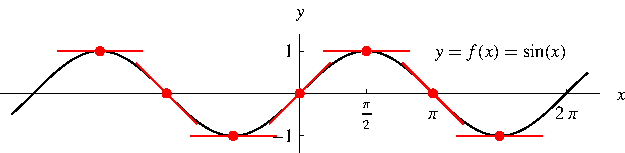
\includegraphics[width=12cm]{derivatives-trig/pictures/03-04-sinh.pdf}%
}%

\ \only<handout:0| 1-2>{%
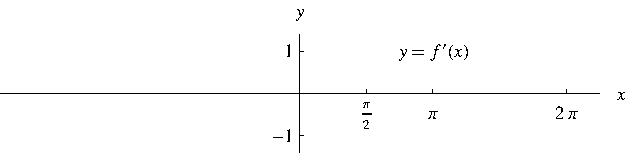
\includegraphics[width=12cm]{derivatives-trig/pictures/03-04-cosa.pdf}%
}%
\only<handout:0| 3-4>{%
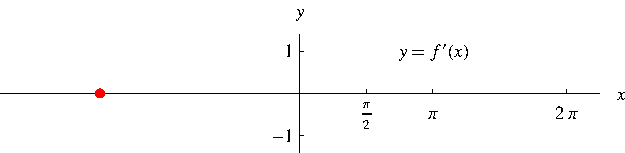
\includegraphics[width=12cm]{derivatives-trig/pictures/03-04-cosb.pdf}%
}%
\only<handout:0| 5-6>{%
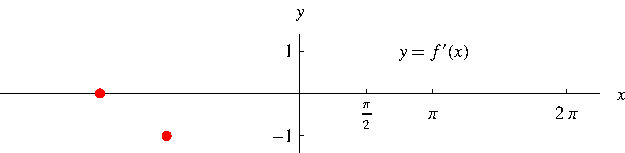
\includegraphics[width=12cm]{derivatives-trig/pictures/03-04-cosc.pdf}%
}%
\only<handout:0| 7-8>{%
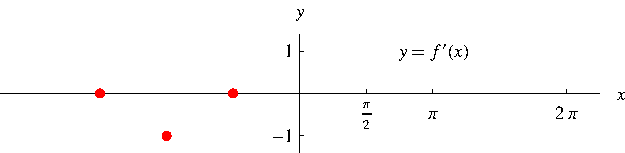
\includegraphics[width=12cm]{derivatives-trig/pictures/03-04-cosd.pdf}%
}%
\only<handout:0| 9-10>{%
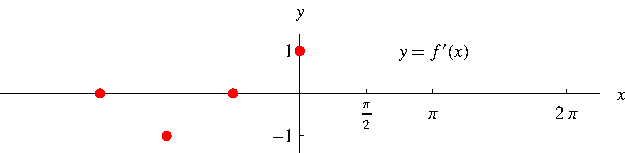
\includegraphics[width=12cm]{derivatives-trig/pictures/03-04-cose.pdf}%
}%
\only<handout:0| 11-12>{%
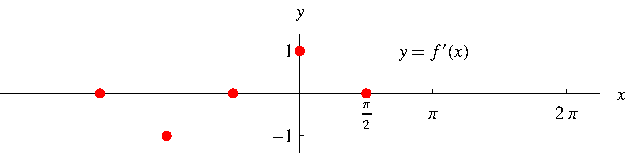
\includegraphics[width=12cm]{derivatives-trig/pictures/03-04-cosf.pdf}%
}%
\only<handout:0| 13-14>{%
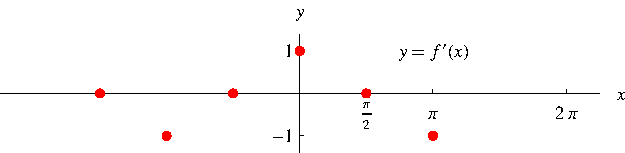
\includegraphics[width=12cm]{derivatives-trig/pictures/03-04-cosg.pdf}%
}%
\only<handout:0| 15-16>{%
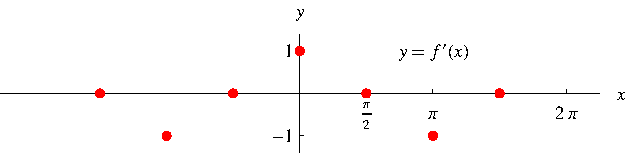
\includegraphics[width=12cm]{derivatives-trig/pictures/03-04-cosh.pdf}%
}%
\only<17->{%
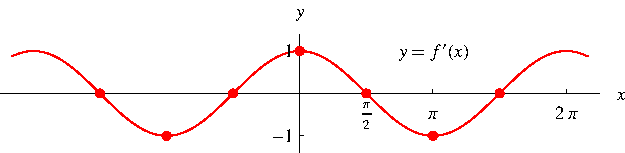
\includegraphics[width=12cm]{derivatives-trig/pictures/03-04-cosi.pdf}%
}%

What is the derivative of $f(x) = \sin x$?  \uncover<16->{It looks like $\cos x$.}
\end{frame}
% end module derivative-sine-graph
